\begin{figure}
    \centering
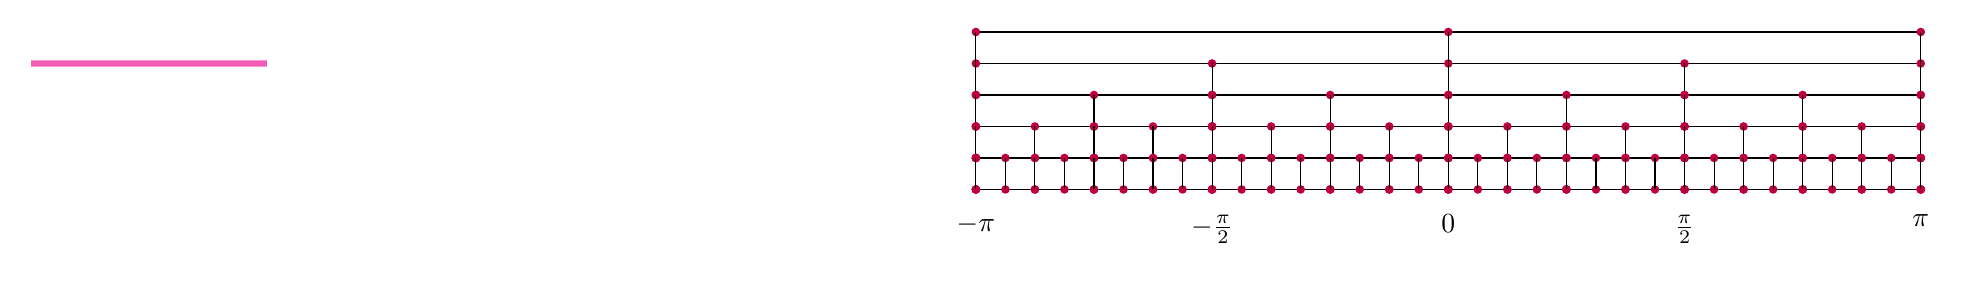
\begin{tikzpicture}[scale=2]
  % Draw horizontal lines
  \draw (0,0) -- (6,0);
  \draw (0,0.2) -- (6,0.2);
  \draw (0,0.4) -- (6,0.4);
  \draw (0,0.6) -- (6,0.6);
  \draw (0,0.8) -- (6,0.8);
  \draw (0,1) -- (6,1);
  
  % Draw marked points and vertical lines
  \foreach \y in {0,0.2,0.4,0.6,0.8,1} {
    \draw (3,\y) node[circle,fill,inner sep=1.1pt, color=purple]{}; % Marked point
    \draw (0,\y) node[circle,fill,inner sep=1.1pt, color=purple]{}; % Marked point
    \draw (6,\y) node[circle,fill,inner sep=1.1pt, color=purple]{}; % Marked point
    \draw (3,\y) -- (3,0); % Vertical line
    \draw (0,\y) -- (0,0); % Vertical line
    \draw (6,\y) -- (6,0); % Vertical line
  }

  \foreach \y in {0,0.2,0.4,0.6,0.8} {
    \draw (1.5,\y) node[circle,fill,inner sep=1.1pt, color=purple]{}; % Marked point
    \draw (4.5,\y) node[circle,fill,inner sep=1.1pt, color=purple]{}; % Marked point
    \draw (4.5,\y) -- (4.5,0); % Vertical line
    \draw (1.5,\y) -- (1.5,0); % Vertical line
  }

  \foreach \y in {0,0.2,0.4,0.6} {
    \pgfmathsetmacro{\z}{6/8}
    \foreach \i in {0,...,8}{
    \pgfmathsetmacro{\x}{\z * \i}
    \draw (\x,\y) node[circle,fill,inner sep=1.1pt, color=purple]{}; % Marked point
    \draw (\x,\y) -- (\x,0); % Vertical line
    }
  }

  \foreach \y in {0,0.2,0.4} {
    \pgfmathsetmacro{\z}{6/16}
    \foreach \i in {0,...,16}{
    \pgfmathsetmacro{\x}{\z * \i}
    \draw (\x,\y) node[circle,fill,inner sep=1.1pt, color=purple]{}; % Marked point
    \draw (\x,\y) -- (\x,0); % Vertical line
    }
  }

  \foreach \y in {0,0.2} {
    \pgfmathsetmacro{\z}{6/32}
    \foreach \i in {0,...,32}{
    \pgfmathsetmacro{\x}{\z * \i}
    \draw (\x,\y) node[circle,fill,inner sep=1.1pt, color=purple]{}; % Marked point
    \draw (\x,\y) -- (\x,0); % Vertical line
    }
  }



  % Label horizontal lines
  \draw (0,-0.1) node[below] {$-\pi$};
  \draw (1.5,-0.1) node[below] {$-\frac \pi 2$};
  \draw (3,-0.1) node[below] {$0$};
  \draw (4.5,-0.1) node[below] {$\frac \pi 2$};
  \draw (6,-0.1) node[below] {$\pi$};

  \draw [magenta,-, double=magenta, double distance=4\pgflinewidth, opacity=0.4,
  ] (-6,0.8) -- (-4.5,0.8);

\end{tikzpicture}
\captionof{figure}{A convenient representation of the dyadic grid in the Böttcher coordinates.
 The horizontal axis is the external ray angle, and the vertical axis is the equipotential $|\psi ^{-1}(z)|$, plotted on a log scale. 
 The rightmost edge is glued to the leftmost edge.
 Stations are marked in red, and the segments connecting adjacent stations are tracks. An express track is a vertical segment, and a peripheral track is horizontal.}
\end{figure}

